\documentclass{article}
\usepackage{graphicx}

\oddsidemargin = -0.25in
\headheight = 12pt
\textheight = 9in
\hoffset = 0pt
\topmargin = -0.5in
\headsep = 25pt
\textwidth = 7in

\title{RT-LAMP assay for detecting lentiviruses}

\begin{document}
\maketitle
%\tableofcontents
%\newpage

\section{Introduction}

Tests for known lentivirus retroviruses with a high viral diversity such as HIV are very specific and could miss divergent HIV strains \cite{bartolo2012hiv}\cite{luft2011hiv}. In \cite{voisset2008human}, a number of studies designing degenerate PCR primers for detecting lentiviruses are reviewed. In \cite{giovine1994absence}, PCR primers targetting a conserved region of the pol gene across five different lentivirus sequences were designed. The goal of the study was to look for evidence of a lentivirus in patients with rhematoid arthritis. \\

\noindent
equine infectious anemia virus (EIAV; Genbank no. M16575) \\
visna-maedi virus (VISNA; Genbank no. M10608) \\
caprine arthritis-encephalitis virus(CAEV; Genbank no. K03327) \\
human immunodeficiency virus type 1 (HIV-I; Genbank no. K03455) \\
HIV-2 (Genbank no. M15390) \\

\noindent
All representative sequences were complete genomes with the exception of CAEV, which was only the pol gene.\\

\noindent
NCBI Genbank search:\\
M16575 M10608 K03327 K03455 M15390\\
https://www.ncbi.nlm.nih.gov/nuccore/M16575,M10608,K03327,K03455,M15390\\
Download file in FASTA format\\
multiple sequence alignment with Clustal O\\

%264
%267

\noindent
The following degenerate PCR primers were used:\\
Forward primer 5' to 3':\\
CAATGGCCMTTVACDGAAGARAAAHTA\\
Reverse primer 5' to 3':\\
TARGGGTAKWGWAAARTATGCATCHCC\\

reverse complement of reverse primer:\\
GGDGATGCATAYTTTWCWMTACCCYTA\\



The degeneracy of a sequence is the number of unique sequence combinations it contains, which can be calculated as d(S) = Π l i=1|x i |.

match % is number of matching nucleotides out of total length\\

\begin{figure}[h!]
\centering
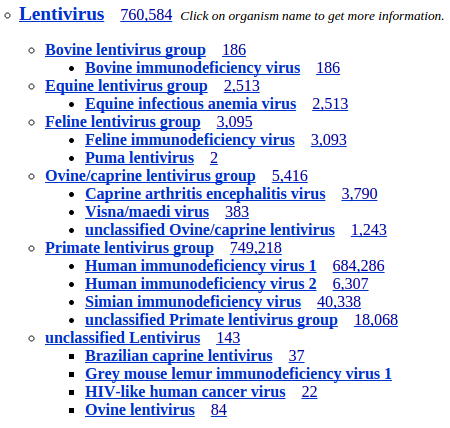
\includegraphics[width=4.5in]{taxonomy_crop.png}
\caption{Lentivirus Taxonomy}
\label{taxonomy}
\end{figure}


A number of RT-LAMP assays using degenerate primer \cite{fukuta2003detection}\cite{nunes2015analysis}

\section{Design}

design constraints balance minimal design/development time, minimal equipment requirements, adequate performance.

Primer design tools:\\
Primer Explorer\\
LAVA\\
\cite{torres2011lava}

Primer validation:\\
eLAMP
\cite{salinas2012electric}

see if simulated analysis matches experimental result from previous study as form of evaluation since eLAMP paper did not verify actual amplification against simulated results.

\subsection{Sample Collection}

minimal sample volume, blood drop from lanclet 

\subsection{Lysis}

\cite{curtis2008rapid}

\subsection{Reaction}



\bibliographystyle{ieeetr}
\bibliography{nucleic_acid_amplification}


\end{document}
